%#!platex main

\chapter{導入}
\label{134138_29Mar06}

本講義では、コンパイラの内部構成について、理論面から実際のプログラムに至
るまでを扱う。

C言語のコンパイラは演習・実験等でよく使っているはずである。このソフトウェ
アは、C言語のプログラムを機械語のプログラムや実行形式ファイル
(\icode{a.out}など)に変換してくれる。一般に{\bfseries コンパイ
ラ}(compiler)とは、「あるプログラミング言語で書かれたプログラムを読み込
んで、別のプログラミング言語による等価なプログラムに翻訳するソフトウェア」
である。翻訳前のプログラミング言語を{\bfseries 原始言語}(source
language)、翻訳後のプログラミング言語を{\bfseries 目的言語}(target
language)という。また、翻訳前のプログラムを{\bfseries 原始プログラ
ム}(source program)、翻訳後のプログラムを{\bfseries 目的プログラ
ム}(target program)という。C言語のコンパイラは、原始言語がC、目的言語が
機械語であるようなコンパイラ\footnote{\icode{gcc}は、C以外の言語(C++など)
も原始言語として扱える。}である。またコンパイラは、原始プログラムを解析し、
その中に文法的な誤りがあれば、そのことをユーザに通知してくれる。

コンパイラの歴史は1950年代にさかのぼる。当時は、コンパイラは実装にひどく
手間のかかるソフトウェアであった。しかし、その後1980年代頃までに、コンパ
イラ設計に関する理論的かつ体系的な手法がいろいろ考案され、コンパイラ実装
の多くの部分は自動で行えるようになった。

したがってコンパイラの設計技法は、情報科学、ハードウェア、ソフトウェアの
3分野が交差するところにあり、関連科目も多岐に渡る。
\begin{description}
 \item[先行科目] 情報処理学、離散数学、プログラミング言語I、プログラミング言語II、計算機アーキテクチャA
 \item[後続科目] 形式言語理論(修士)
\end{description}
このほか、この講義ではプログラム例の記述にC言語を用いる。そのため、講義全
般を通してC言語の知識が必要になる。

この講義は
\cite{aho86:_compiler}\cite{aho07:_compil_princ_techn_tools_secon_edition}
\cite{湯浅01}を基にしている。ただし、分量が膨大であり、かつ難解な部分も多
いので、基礎的な部分を抜粋して構成している\footnote{本テキスト中の例につ
いてはこれらの書籍からの引用がかなり多く、学外関係者に流布すると著作権上
問題がある。本資料の利用は学内関係者のみにとどめておいていただきたい。}。その他、
\cite{ホップクロフト03:automaton}\cite{中田99}\cite{カーニハン89}などを適
宜参照している。

\section{コンパイラの構成}
\label{134201_29Mar06}

今後の講義の流れを知っておくために、例を用いてコンパイラの内部構成を簡単
に説明することにしよう。次のCプログラム(\icode{simple.c})を考える。

\begin{quote}
\lstinputlisting{code/simple.c}
\end{quote}

\begin{figure}
 \lstinputlisting[language={[x86masm]Assembler},numbers=left,xleftmargin=100pt]{code/simple.s}
 \caption{i386機械語命令の例}
 \label{143232_11Apr06}
\end{figure}

コンパイラは\icode{simple.c}の内容を解析し、例えば図\ref{143232_11Apr06}
のような機械語列を生成する\footnote{i386アーキテクチャを仮定している。}。
なお、本当の機械語列は、それぞれのシンボルを0/1の列で置き換えたものになる。

各機械語命令は、CPUによって直接解釈実行することができる。
\icode{simple.c}をコンパイルして得られた実行形式ファイル(\icode{a.out}な
ど)を実行すると、この機械語命令列が主記憶上にロードされ、CPUがそれを順次
解釈して実行していく。各行の意味はだいたい次のようになっている。
\begin{itemize}
 \item 3行目…\icode{\_main}という目印(ラベル)づけ。\icode{main}関数に対
       応している。
 \item 4-6行目…\icode{main}関数の呼び出し処理。このとき、
       \icode{-16(\%ebp)}番地から4バイトの領域に局所変数\icode{x}が、
       \icode{-12(\%ebp)}番地から4バイトの領域に局所変数\icode{y}がそれぞ
       れ割り当てられる。
 \item 7行目…\icode{y}の領域に\icode{\$1}、すなわち定数1がセットされる。
 \item 8行目…\icode{y}の領域の値がレジスタ\icode{\%eax}にセットされる。
 \item 9行目…レジスタ\icode{\%eax}の値に定数20が加えられる。
 \item 10行目…レジスタ\icode{\%eax}の値が\icode{x}の領域にセットされる。
 \item 11-13行目…\icode{main}関数の終了処理\footnote{11-12行目は
       \icode{leave}という1つの機械語命令にまとめられていることもある。}。
\end{itemize}

この講義で扱う内容を整理すると次のようになる。
\begin{enumerate}
 \item 原始プログラム(上の例ではCプログラム)から目的プログラム(上の例
       では機械語列)を生成するアルゴリズム\label{195753_28Mar06}
 \item \ref{195753_28Mar06}を実現するプログラム
       \label{195816_28Mar06}
 \item \ref{195816_28Mar06}を自動的に生成するアルゴリズム/手法
       \label{200119_28Mar06}
\end{enumerate}
\ref{195753_28Mar06}と\ref{200119_28Mar06}の違いに充分留意されたい。

さて、コンパイラは大きく分けて以下の2つの部分から構成される。
\begin{description}
 \item[解析部] 原始プログラムを解析し、コンパイラ内部で処理するためのデー
	    タ構造({\bfseries 中間表現})を作る。文字列としての原始プロ
	    グラムからプログラムの最小意味単位({\bfseries トークン},
	    token)を切り出す{\bfseries 字句解析}(lexical analysis)部、
	    トークン列からプログラムの意味構造を解析する{\bfseries 構文解
	    析}(syntax analysis)部、型の検査など構文解析部では行
	    えないプログラム解析を行う{\bfseries 意味解析}(semantic
	    analysis)部の3つの部分からなる。また、先の例の\icode{main},
	    \icode{x}, \icode{y}など、ユーザが定義した変数や関数の列挙も
	    この段階で行われる。
 \item[合成部] 解析部で作った中間表現を基に、目的プログラムを合成する。場
	    合によっては、実行速度を上げるために、合成したプログラムをさ
	    らに加工することもある({\bfseries 最適化}, optimization)。
\end{description}

コンパイラは、最初は原始プログラムを単なる文字の並びとして扱う。先の例で
言えば、次のような文字の並びとして扱う(\verb|\n|は改行文字を表す)。
\begin{quote}
\verb|int main()\n{\n int x;\n int y = 1;\n x = y + 20;\n}\n|
\end{quote}
ここからC言語として意味のある文字列を切り出すのが字句解析部である。結果は
次のような文字列の並びになる\footnote{後で述べるように、実際には、出力す
るのはそれぞれの文字列を抽象化した記号、すなわちトークンである。また、一
度にこのような並びをまとめて出力するのではなく、字句解析部に要求があるた
びに一つずつ切り出して出力する。}。空白や改行文字など、C言語として意味の
ない文字列は出力されていないことに注意しておいてほしい。
\begin{quote}
 \verb|int|, \verb|main|, \verb|(|, \verb|)|, \verb|{|, \verb|int|,
 \verb|x|, \verb|;|, \verb|int|, \verb|y|, \verb|=|, \verb|1|, 
 \verb|;|, \verb|x|, \verb|=|, \verb|y|, \verb|+|, \verb|20|, \verb|;|,
 \verb|}|
\end{quote}

この並びを、プログラミング言語の文法に従ってグループ化し、意味のまとまり
を解析するのが構文解析部である。例えば、セミコロン \verb|;| はC言語の文の区
切りであり、セミコロンで囲まれた次の部分は一つのまとまりになる。
\begin{quote}
 \verb|x|, \verb|=|, \verb|y|, \verb|+|, \verb|20|
\end{quote}
これはさらに\verb|x|, \verb|=|, \verb|y| \verb|+| \verb|20|という3つの部
分にグループ化でき、さらに最後の部分は\verb|y|, \verb|+|, \verb|20|という
3つの部分にグループ化できる。このように、グループ化した結果、つまり構文解
析の結果は通常グループの入れ子になり、木で表現するのが一般的である(図
\ref{112135_29Mar06})。論理的には、これが構文解析部の出力データ構造にな
る。

\begin{figure}
 \begin{center}
  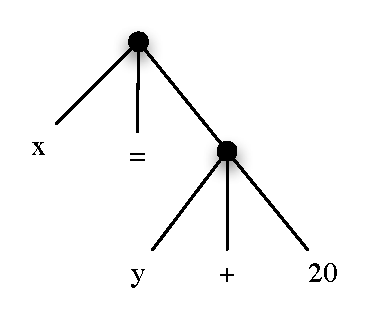
\includegraphics[scale=0.8]{figure/tree_structure.pdf}
 \end{center}
 \caption{{\sffamily x = y + 20}を表す木構造}
 \label{112135_29Mar06}
\end{figure}

この木には、型の情報など、プログラム実行のための重要な情報がいくつか含ま
れていない。これを補うのが意味解析部である。定数や変数の型変換などは意味
解析部で適宜処理される。その結果、構文解析部の出力の木に修正が加えられる
こともある。

ここまでで得られた木構造を基にして、目的プログラムが合成される。その際、
いきなり目的プログラムを合成するのではなく、いったん擬似的な機械語列を生
成してから実際の目的プログラムに変換するほうが考えやすい。例えば、
{\sffamily x = y + 20}に対して、新たな変数\icode{temp1}, \icode{temp2}を
導入し、次のような擬似機械語列を考える。
\begin{quote}
\begin{verbatim}
	temp1 = y
	temp2 = temp1 + 20
	x = temp2
\end{verbatim}
\end{quote}
すると、先に示した目的プログラムとの対応がとりやすくなることが分かるだろ
う。この擬似機械語列に対して、変数\icode{temp1}, \icode{temp2}にレジスタ
\icode{\%eax}を、\icode{x}に番地\icode{-16(\%ebp)}を、\icode{y}に番地
\icode{-12(\%ebp)}をそれぞれ割り当てると、先に示した目的プログラムが生成
できる。レジスタや番地の割り当て、関数呼び出し時の処理コードの追加なども
合成部で行われる。

なお、ここで述べたコンパイラの構成はもっとも基本的なものである。実際のコ
ンパイラ設計ではこの構成に厳密には従わないことも多々ある。

\section{練習問題}

\begin{exercise}
\label{ex:intro01}
 \icode{gcc}は、\icode{-s}オプションをつけることで機械語命令列を出力させ
 ることができる。簡単なC言語プログラムを各自で書き、どのような機械語命令
 列が出力されるか、試してみよ。
\end{exercise}
\begin{exercise}
\label{ex:intro02}
 次のC言語の文を、C言語として意味のある文字列に分解せよ。
 \begin{quote}
  \verb|x = 0; while (i < 100) { x += i; i++; }|
 \end{quote}
\end{exercise}
